\begin{figure}
\begin{subfigure}{0.31\textwidth}
\centering
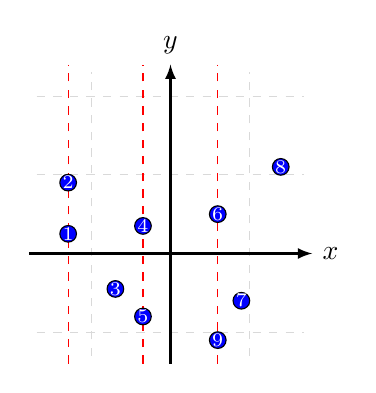
\begin{tikzpicture}
        \draw[help lines, color=gray!30, dashed] (-1.7,-1.3) grid (1.7,2.3);
    \draw[-latex, thick] (-1.8,0)--(1.8,0) node[right]{$x$};
    \draw[-latex, thick] (0,-1.4)--(0,2.4) node[above]{$y$};

    \draw[-, dashed, red] (-1.3, -1.4) -- (-1.3, 2.4);
    \draw[-, dashed, red] (-0.35, -1.4) -- (-0.35, 2.4);
    \draw[-, dashed, red] (0.6, -1.4) -- (0.6, 2.4);
    \node[draw, circle, fill=blue, text=white, inner sep=0pt, minimum size=5pt] (p1) at (-1.3, 0.25) {\scriptsize $1$};
    \node[draw, circle, fill=blue, text=white, inner sep=0pt, minimum size=5pt] (p2) at (-1.3, 0.9) {\scriptsize $2$};
    \node[draw, circle, fill=blue, text=white, inner sep=0pt, minimum size=5pt] (p3) at (-0.7, -0.45) {\scriptsize $3$};
    \node[draw, circle, fill=blue, text=white, inner sep=0pt, minimum size=5pt] (p4) at (-0.35, 0.35) {\scriptsize $4$};
    \node[draw, circle, fill=blue, text=white, inner sep=0pt, minimum size=5pt] (p5) at (-0.35, -0.8) {\scriptsize $5$};
    \node[draw, circle, fill=blue, text=white, inner sep=0pt, minimum size=5pt] (p6) at (0.6, 0.5) {\scriptsize $6$};
    \node[draw, circle, fill=blue, text=white, inner sep=0pt, minimum size=5pt] (p7) at (0.9, -0.6) {\scriptsize $7$};
    \node[draw, circle, fill=blue, text=white, inner sep=0pt, minimum size=5pt] (p8) at (1.4, 1.1) {\scriptsize $8$};
    \node[draw, circle, fill=blue, text=white, inner sep=0pt, minimum size=5pt] (p9) at (0.6, -1.1) {\scriptsize $9$};
\end{tikzpicture}
\caption{The original list of points.\\\phantom{x}\\\phantom{x}}\label{fig:symmetry-breaking-1}
\end{subfigure}
\hfil
\begin{subfigure}{0.31\textwidth}
    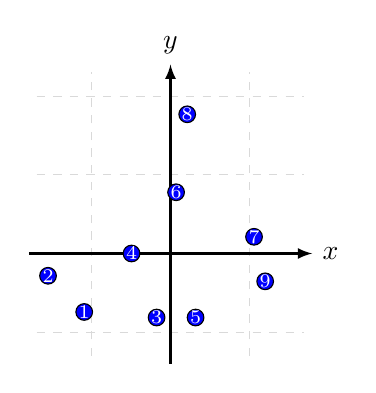
\begin{tikzpicture}
        \draw[help lines, color=gray!30, dashed] (-1.7,-1.3) grid (1.7,2.3);
    \draw[-latex, thick] (-1.8,0)--(1.8,0) node[right]{$x$};
    \draw[-latex, thick] (0,-1.4)--(0,2.4) node[above]{$y$};
    
        \node[draw, circle, fill=blue, text=white, inner sep=0pt, minimum size=5pt] (p1) at (-1.09601563215555, -0.7424619411597272) {\scriptsize $1$};
        \node[draw, circle, fill=blue, text=white, inner sep=0pt, minimum size=5pt] (p2) at (-1.5556349648261614, -0.28284245828783905) {\scriptsize $2$};
        \node[draw, circle, fill=blue, text=white, inner sep=0pt, minimum size=5pt] (p3) at (-0.17677682816699475, -0.8131727694796578) {\scriptsize $3$};
        \node[draw, circle, fill=blue, text=white, inner sep=0pt, minimum size=5pt] (p4) at (-0.49497474683057663, 8.087761060870946e-08) {\scriptsize $4$};
        \node[draw, circle, fill=blue, text=white, inner sep=0pt, minimum size=5pt] (p5) at (0.3181979186635819, -0.8131728503572684) {\scriptsize $5$};
        \node[draw, circle, fill=blue, text=white, inner sep=0pt, minimum size=5pt] (p6) at (0.07071080521204193, 0.7778174477512475) {\scriptsize $6$};
        \node[draw, circle, fill=blue, text=white, inner sep=0pt, minimum size=5pt] (p7) at (1.0606602064416402, 0.21213186104679588) {\scriptsize $7$};
        \node[draw, circle, fill=blue, text=white, inner sep=0pt, minimum size=5pt] (p8) at (0.21213232320457065, 1.767766918304512) {\scriptsize $8$};
        \node[draw, circle, fill=blue, text=white, inner sep=0pt, minimum size=5pt] (p9) at (1.202081470247393, -0.3535535870103234) {\scriptsize $9$};
    \end{tikzpicture}

\caption{All $x$-coordinates are different after rotating by $45^\circ$. We show such an angle always exists.}\label{fig:symmetry-breaking-2}
\end{subfigure}
\hfil
%
%\vspace{0.5cm}
%
\begin{subfigure}{0.31\textwidth}
    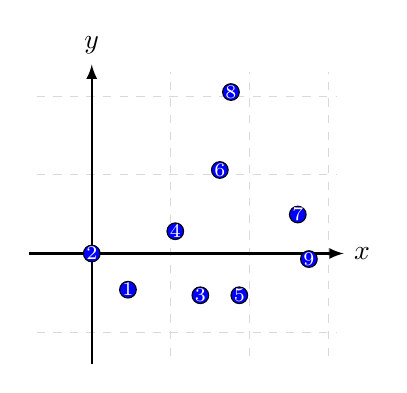
\begin{tikzpicture}
            \draw[help lines, color=gray!30, dashed] (-0.7,-1.3) grid (3.1,2.3);
    \draw[-latex, thick] (-0.8,0)--(3.2,0) node[right]{$x$};
    \draw[-latex, thick] (0,-1.4)--(0,2.4) node[above]{$y$};
    
    
%        \draw[help lines, color=gray!30, dashed] (-1,-0.9) grid (2.9,2.4);
%        \draw[-latex, thick] (-1,0)--(4,0) node[right]{$x$};
%        \draw[-latex, thick] (0,-1)--(0,2.5) node[above]{$y$};
    
        \node[draw, circle, fill=blue, text=white, inner sep=0pt, minimum size=5pt] (p1) at (0.4596193326706113, -0.45961948287188814) {\scriptsize $1$};
        \node[draw, circle, fill=blue, text=white, inner sep=0pt, minimum size=5pt] (p2) at (0.0, 0.0) {\scriptsize $2$};
        \node[draw, circle, fill=blue, text=white, inner sep=0pt, minimum size=5pt] (p3) at (1.3788581366591666, -0.5303303111918187) {\scriptsize $3$};
        \node[draw, circle, fill=blue, text=white, inner sep=0pt, minimum size=5pt] (p4) at (1.0606602179955846, 0.28284253916544966) {\scriptsize $4$};
        \node[draw, circle, fill=blue, text=white, inner sep=0pt, minimum size=5pt] (p5) at (1.8738328834897433, -0.5303303920694293) {\scriptsize $5$};
        \node[draw, circle, fill=blue, text=white, inner sep=0pt, minimum size=5pt] (p6) at (1.6263457700382034, 1.0606599060390867) {\scriptsize $6$};
        \node[draw, circle, fill=blue, text=white, inner sep=0pt, minimum size=5pt] (p7) at (2.6162951712678018, 0.4949743193346349) {\scriptsize $7$};
        \node[draw, circle, fill=blue, text=white, inner sep=0pt, minimum size=5pt] (p8) at (1.767767288030732, 2.0506093765923508) {\scriptsize $8$};
        \node[draw, circle, fill=blue, text=white, inner sep=0pt, minimum size=5pt] (p9) at (2.7577164350735544, -0.07071112872248436) {\scriptsize $9$};
    \end{tikzpicture}

\caption{After translating the leftmost point is at $(0,0)$.\\\phantom{x}}\label{fig:symmetry-breaking-3}
\end{subfigure}

\begin{subfigure}{0.31\textwidth}
    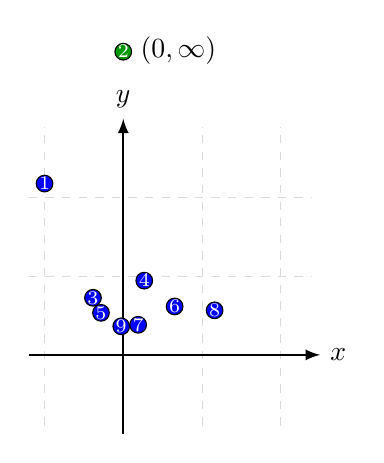
\begin{tikzpicture}
        \draw[help lines, color=gray!30, dashed] (-1.2,-0.9) grid (2.4,2.9);
        \draw[-latex, thick] (-1.2,0)--(2.5,0) node[right]{$x$};
        \draw[-latex, thick] (0,-1)--(0,3) node[above]{$y$};
    
        \node[draw, circle, fill=blue, text=white, inner sep=0pt, minimum size=5pt] (p1) at (-1.00000032679495, 2.1757135283877527) {\scriptsize $1$};
        \node[draw, circle, fill=green!60!black, text=white, inner sep=0pt, minimum size=5pt, label={[xshift=0.7cm, yshift=-0.4cm]$(0, \infty)$}] (p2) at (0, 3.85) {\scriptsize $2$};
        \node[draw, circle, fill=blue, text=white, inner sep=0pt, minimum size=5pt] (p3) at (-0.3846155721840648, 0.7252377698715973) {\scriptsize $3$};
        \node[draw, circle, fill=blue, text=white, inner sep=0pt, minimum size=5pt] (p4) at (0.2666664916498519, 0.9428090005013866) {\scriptsize $4$};
        \node[draw, circle, fill=blue, text=white, inner sep=0pt, minimum size=5pt] (p5) at (-0.2830190444100679, 0.5336655199142649) {\scriptsize $5$};
        \node[draw, circle, fill=blue, text=white, inner sep=0pt, minimum size=5pt] (p6) at (0.6521736801480853, 0.6148753963780468) {\scriptsize $6$};
        \node[draw, circle, fill=blue, text=white, inner sep=0pt, minimum size=5pt] (p7) at (0.1891890199433349, 0.3822198699068886) {\scriptsize $7$};
        \node[draw, circle, fill=blue, text=white, inner sep=0pt, minimum size=5pt] (p8) at (1.1599996167350177, 0.5656853177286622) {\scriptsize $8$};
        \node[draw, circle, fill=blue, text=white, inner sep=0pt, minimum size=5pt] (p9) at (-0.025641189145902285, 0.3626188636662086) {\scriptsize $9$};
       
    \end{tikzpicture}

\caption{Result after applying the map $(x, y) \mapsto (y/x, 1/x)$.}\label{fig:symmetry-breaking-4}
\end{subfigure}
\hfil
%
%\vspace{0.5cm}
%
\begin{subfigure}{0.31\textwidth}
    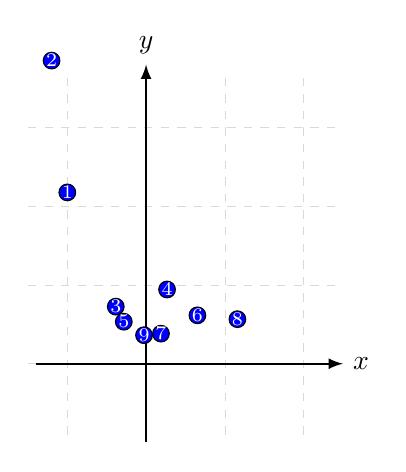
\begin{tikzpicture}
        \draw[help lines, color=gray!30, dashed] (-1.5,-0.9) grid (2.4,3.7);
        \draw[-latex, thick] (-1.4,0)--(2.5,0) node[right]{$x$};
        \draw[-latex, thick] (0,-1)--(0,3.8) node[above]{$y$};
    
           
        \node[draw, circle, fill=blue, text=white, inner sep=0pt, minimum size=5pt] (p1) at (-1.00000032679495, 2.1757135283877527) {\scriptsize $1$};
        \node[draw, circle, fill=blue, text=white, inner sep=0pt, minimum size=5pt] (p2) at (-1.2, 3.85) {\scriptsize $2$};
        \node[draw, circle, fill=blue, text=white, inner sep=0pt, minimum size=5pt] (p3) at (-0.3846155721840648, 0.7252377698715973) {\scriptsize $3$};
        \node[draw, circle, fill=blue, text=white, inner sep=0pt, minimum size=5pt] (p4) at (0.2666664916498519, 0.9428090005013866) {\scriptsize $4$};
        \node[draw, circle, fill=blue, text=white, inner sep=0pt, minimum size=5pt] (p5) at (-0.2830190444100679, 0.5336655199142649) {\scriptsize $5$};
        \node[draw, circle, fill=blue, text=white, inner sep=0pt, minimum size=5pt] (p6) at (0.6521736801480853, 0.6148753963780468) {\scriptsize $6$};
        \node[draw, circle, fill=blue, text=white, inner sep=0pt, minimum size=5pt] (p7) at (0.1891890199433349, 0.3822198699068886) {\scriptsize $7$};
        \node[draw, circle, fill=blue, text=white, inner sep=0pt, minimum size=5pt] (p8) at (1.1599996167350177, 0.5656853177286622) {\scriptsize $8$};
        \node[draw, circle, fill=blue, text=white, inner sep=0pt, minimum size=5pt] (p9) at (-0.025641189145902285, 0.3626188636662086) {\scriptsize $9$};
       
       
    \end{tikzpicture}

\caption{Point $2$ is brought back into the real plane.}\label{fig:symmetry-breaking-5}
\end{subfigure}
\hfil
\begin{subfigure}{0.31\textwidth}
    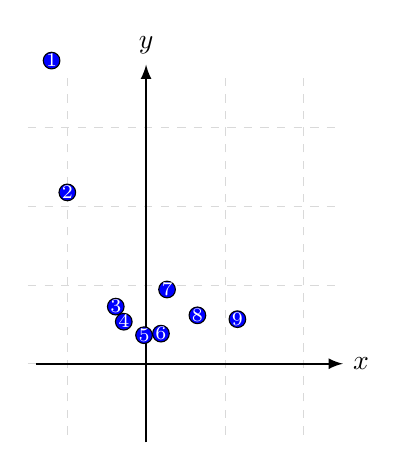
\begin{tikzpicture}
        \draw[help lines, color=gray!30, dashed] (-1.5,-0.9) grid (2.4,3.7);
        \draw[-latex, thick] (-1.4,0)--(2.5,0) node[right]{$x$};
        \draw[-latex, thick] (0,-1)--(0,3.8) node[above]{$y$};
    
           
        \node[draw, circle, fill=blue, text=white, inner sep=0pt, minimum size=5pt] (p1) at (-1.2, 3.85) {\scriptsize $1$};
        \node[draw, circle, fill=blue, text=white, inner sep=0pt, minimum size=5pt] (p2) at (-1.00000032679495, 2.1757135283877527) {\scriptsize $2$};
        \node[draw, circle, fill=blue, text=white, inner sep=0pt, minimum size=5pt] (p3) at (-0.3846155721840648, 0.7252377698715973) {\scriptsize $3$};
        \node[draw, circle, fill=blue, text=white, inner sep=0pt, minimum size=5pt] (p4) at (-0.2830190444100679, 0.5336655199142649) {\scriptsize $4$};
        \node[draw, circle, fill=blue, text=white, inner sep=0pt, minimum size=5pt] (p5) at (-0.025641189145902285, 0.3626188636662086) {\scriptsize $5$};
        \node[draw, circle, fill=blue, text=white, inner sep=0pt, minimum size=5pt] (p6) at (0.1891890199433349, 0.3822198699068886) {\scriptsize $6$};
        \node[draw, circle, fill=blue, text=white, inner sep=0pt, minimum size=5pt] (p7) at (0.2666664916498519, 0.9428090005013866) {\scriptsize $7$};
        \node[draw, circle, fill=blue, text=white, inner sep=0pt, minimum size=5pt] (p8) at (0.6521736801480853, 0.6148753963780468) {\scriptsize $8$};
        \node[draw, circle, fill=blue, text=white, inner sep=0pt, minimum size=5pt] (p9) at (1.1599996167350177, 0.5656853177286622) {\scriptsize $9$};
       
    \end{tikzpicture}

\caption{Points are relabeled from left to right.}\label{fig:symmetry-breaking-6}
\end{subfigure}



\caption{Illustration of the proof of the main symmetry breaking theorem. For simplicity we have ommited the illustration of the \emph{left-to-right} property. }\label{fig:symmetry-breaking}
\end{figure}